\documentclass[12pt, a4paper]{article}
\usepackage[utf8x]{inputenc}
\usepackage{indentfirst} %indentace prvního odstavce
\usepackage{mathtools}
\usepackage{amsfonts}
\usepackage{amsmath}
\usepackage{amssymb}
\usepackage{graphicx}
\usepackage{enumitem}
\usepackage{subfig}
\usepackage{float}
\usepackage[czech]{babel}

\begin{document}

\section{}
Definujeme vektor stavu HP pokémonů jako $h(t) = (h_1(t), h_2(t))^T$, kde $h_1(t)$ značí hodnotu HP Pikachu po kole $t$ a $h_2(t)$ hodnotu HP Charmandera po kole $t$. Víme, že $h_1(0)=100$ a $h_2(0)=50$. Ze zadání je zřejmé, že platí:
\begin{gather*}
A = \begin{pmatrix}
0.95 & -0.2\\
-0.1 & 1.1
\end{pmatrix}\\
h(t+1) = A \cdot h(t)
\end{gather*}

Vidíme, že toto je předpis pro lineární dynamický systém a tedy zřejmě platí $h(t) = A^{t}\cdot h(0)$.
Matice A je diagonalizovatelná, protože její vlastní vektory tvoří bázi $\mathbb{R}^2$. Platí:
\begin{gather*}
R = \begin{pmatrix}
0.647994 & -0.920202\\
-0.761646 & -0.391445
\end{pmatrix},
D = \begin{pmatrix}
1.18508 & 0\\
0 & 0.864922
\end{pmatrix}\\
A = R \cdot D \cdot R^{-1}
\end{gather*}

Matice $R$ je matice přechodu z báze $B$ tvořené vlastnímy vektory $A$ ke kanonické bázi ($K$) a $R^{-1}$ naopak. Z lineární algebry víme, že platí $[h(t)]_B = D^t \cdot [h(0)]_B$, kde $[\cdot]_B$ značí souřadnice vektorů v bázi B. Dále platí $h(t) = [h(t)]_K= R \cdot [h(t)]_B$ a $[h(0)]_B = R^{-1} \cdot [h(0)]_K = h(0)$. Dosadíme-li:
\begin{gather*}
h(t) = R \cdot [h(t)]_B = R \cdot D^t \cdot [h(0)]_B =  R \cdot D^t \cdot R^{-1} \cdot h(0) \text{ kde }\\
\end{gather*}
Po dosazení a vyčíslený máme explicitní vzorec pro $h(t)$:
\begin{gather*}
h(t) = \begin{pmatrix}
h_1(t)\\
h_2(t)
\end{pmatrix}\approx
\begin{pmatrix}
104.661 \cdot 0.864922^t - 4.66082 \cdot 1.18508^t\\
44.5217 \cdot 0.864922^t - 5.47828 \cdot 1.18508^t\\
\end{pmatrix}
\end{gather*}

Po 9. kole ($t=9$) má Pikachu HP $h_1(9) \approx 6.864$ a Charmander $h_2(9) \approx 37.317$. V po 10. kole by bylo Pikachu mrtvé s $h_1(10) \approx -0.942$. Potřebujeme utéct po 9. kole.

\section{}
Jestliže máme přístup k mapě a máme možnost kreslit kružnice dané délky, tak je úkol jednoduchý. Jednoduše nalezeme průnik 3 kružnic viz obrázek:
\begin{figure}[H]
  \centering
  \subfloat[]{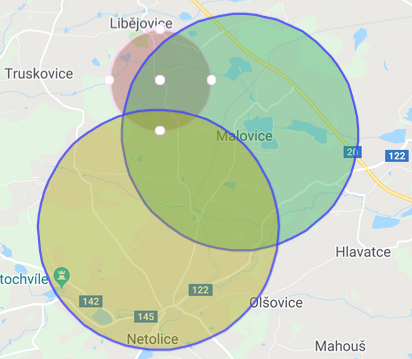
\includegraphics[width=0.4\textwidth]{obr_1.png}\label{fig:f1}}
  \hfill
  \subfloat[]{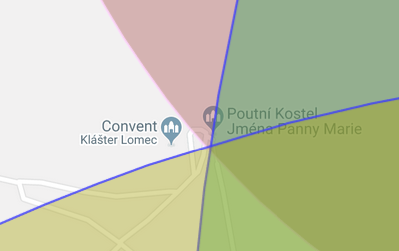
\includegraphics[width=0.4\textwidth]{obr_2.png}\label{fig:f2}}
\end{figure}

To odpovídá zhruba místu \uv{Poutní Kostel Jména Panny Marie} (souřadnice 49°05'44.3"N 14°11'15.3"E). Pokud nemáme přístup k těmto technologiím, tak předpokládáme, že máme přístup k danému souřadnicovému systému na mapě.
\begin{figure}[h]
  \centering
  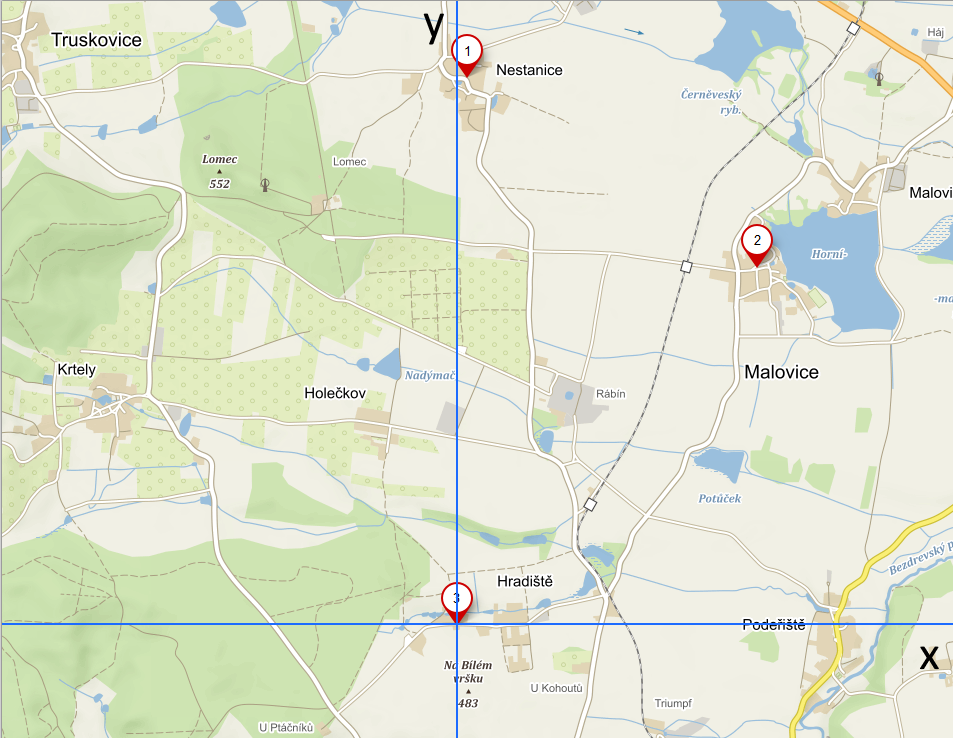
\includegraphics[width=0.8\textwidth]{obr_3.png}
\end{figure}

Kaplička v Hradišti má souřadnice $(x_1, y_1) = (0, 0)^T$, v Malovicích $(x_2, y_2) = (1884, 2235)^T$ a v Nestánicích $(x_3, y_3) = (63, 3423)^T$. Hodnoty souřadnic jsou v metrech. Označme neznámé souřadnice místa $m=(x, y)^T$ a naměřené vzdálenosti od příslušných kapliček $d_1 = 2758, d_2 = 2716, d_3=1171$. Předpokládáme, že platí
\begin{gather*}
(x-x_1)^2 + (y-y_1)^2 = d_1^2\\
(x-x_2)^2 + (y-y_2)^2 = d_2^2\\
(x-x_3)^2 + (y-y_3)^2 = d_3^2
\end{gather*}

Odečteme-li například druhou a třetí rovnici od první dostaneme 2 lineární rovnice $x_1 = y_1 = 0 $:
\begin{gather*}
2x(x_2 - x_1)+2y(y_2 - y_1) = d_1^2 - d_2^2 + x_2^2+y_2^2\\
2x(x_3 - x_1)+2y(y_3 - y_1) = d_1^2 - d_3^2 + x_3^2+y_3^2
\end{gather*}

vyjádřeno maticově
\begin{gather*}
\begin{pmatrix}
2(x_2 - x_1) & 2(y_2 - y_1)\\
2(x_3 - x_1) & 2(y_3 - y_1)\\
\end{pmatrix} \cdot 
\begin{pmatrix}
x\\
y
\end{pmatrix} = 
\begin{pmatrix}
d_1^2 - d_2^2 + x_2^2+y_2^2\\
d_1^2 - d_3^2 + x_3^2+y_3^2\\
\end{pmatrix}
\end{gather*}

Všechny hodnoty kromě $x,y$ známe, tudíž můžeme danou soustavu vyřešit metodou nejmenších čtverců. Výsledek je $m=(-800.296, 2637.61)$, to jsou souřadnice daného místa v naší souřadné soustavě. Výsledek je nečekaně přesný, na to že souřadnice míst čteme \uv{podle oka} viz obrázky.
\begin{figure}[H]
  \centering
  \subfloat[]{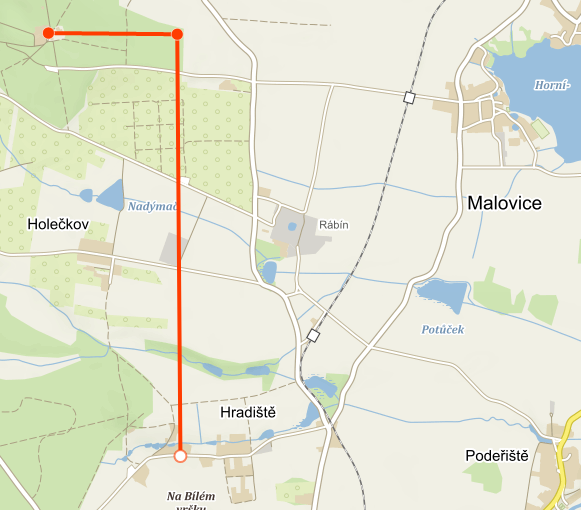
\includegraphics[width=0.4\textwidth]{obr_4.png}\label{fig:f1}}
  \hfill
  \subfloat[]{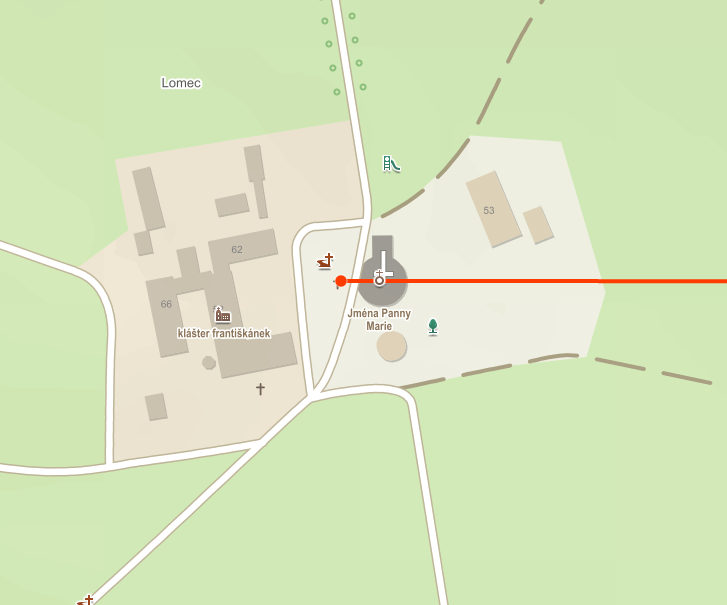
\includegraphics[width=0.4\textwidth]{obr_5.png}\label{fig:f2}}
\end{figure}
\section{}
\subsection{}
$\forall x \in \mathbb{R}^n : x^T A x = x^T B x \iff x^T (A-B) x = 0$. Víme, že $A,B$ jsou symetrické, takže i $(A-B)$ je symetrická matice, tudíž je ortogonálně diagonalizovatelná. Takže existuje $P \in \mathbb{R}^{n \times n}$ ortogonální a $D \in \mathbb{R}^{n \times n}$ diagonální tž. $(A-B) = PDP^T$. $P$ je regulární a tudíž $\forall x \ \exists! y: y=P^Tx$. Tudíž můžeme psát ekvivaletně, že $\forall y \in \mathbb{R}^n: y^T D y = 0$. Pokud za $y$ dosadíme vektory kanonické báze, tak vidíme, že musí platit, že $D = 0$ a tedy i $(A-B) \iff A = B$.

\subsection{}
$P$ pozitivně definitní $\implies$ $P$ je regulární viz LA. Tedy vždy existuje $P^{-1}, Q^{-1}$.
\begin{enumerate}[label=(\alph*)]
\item $P$ regulární tedy opět můžeme přeznačit $y = Px$ a víme, že $y=0 \iff x=0$. $P^{-1}$ je poz. def., protože z definice + dosazení + $P$ symetrická: $\forall y \neq 0: y^T P^{-1} y = x^T P^T P^{-1} P x = x^T P^T x = x^T P x > 0$
\item Pro pozitivně definitní matici $A$ existuje právě jedna matice $\sqrt{A}$ tž. $A = \sqrt{A}^2$. Protože $A$ je poz. def. je ortogonálně diagonalizovatelná s kladnými čisly na diagonále v příslušné diag. matici. Tedy $A = UDU^T$, položme $\sqrt{A}=U \sqrt{D} U^T \implies \sqrt{A}^2 = (U \sqrt{D} U^T)(U \sqrt{D} U^T) = U \sqrt{D} \sqrt{D} U^T = A$. Z definice je zřejmé, že $\sqrt{A}$ je také pozitivně definitní, protože její vlastní čísla jsou kladná (odmocniny kladných čísel).

Nejprve tvrzení dokážeme pro $Q = I$. Víme, že $\forall x: x^T P x \geq x^T Q x = x^T I x$. Nechť $P = A^2$: $x^T P^{-1} x = x^T A^{-1} A^{-1} x = x^T A^{{-1}^T} A^{-1} x = (A^{-1}x)^T I (A^{-1}x) \stackrel{\text{předpoklad}}{\leq} =  (A^{-1}x)^T P (A^{-1}x)=  (A^{-1}x)^T AA (A^{-1}x)=x^T I x$. Dokázali jsme, že $I \preceq P \implies P^{-1} \preceq I$.

Nechť $X$ pozitivně definitní, pak platí $Q \preceq P \implies XQX \preceq XPX$, protože $X$ je regulární (bijekce). Položíme $y= Xx$ a nerovnost stále platí. Nechť $Q = B^2$, nyní $Q$ obecná pozitivně definitní matice. Máme $Q \preceq P \iff BB \preceq P$, položme $X \coloneqq B^{-1}$, potom máme $I \preceq B^{-1}PB^{-1}$. Z již dokázaného máme $(B^{-1}PB^{-1})^{-1} \preceq I^{-1} \iff \\BP^{-1}B \preceq I$. $X \coloneqq B^{-1} \implies P^{-1} \preceq Q^{-1}$.

\item Toto tvrzení neplatí. Protipříklad:
\begin{gather*}
P = \begin{pmatrix}
1/3 & 1/3\\
1/3 & 1/3
\end{pmatrix},
Q = \begin{pmatrix}
-1/2 & -1/2\\
-1/2 & -1/2
\end{pmatrix}
\\
P-Q = \begin{pmatrix}
5/6 & 5/6\\
5/6 & 5/6
\end{pmatrix} \text{ je poz. semidef.}\\
P^2-Q^2 = \begin{pmatrix}
-5/18 & -5/18\\
-5/18 & -5/18
\end{pmatrix} \text{ zřejmě není poz. semidef.}
\end{gather*}
\end{enumerate}

\subsection{}
$\sum_{i=1}^{n-1} (x_{i+1}-x_{i})^2 = x^2_n + 2x^2_{n-1} + \dots 2x^2_2 + x^2_1 -2(x_nx_{n-1} + x_{n-1}x_{n-2} + \dots x_2x_1)$. Tedy je vidět, že
\begin{gather*}
P = \begin{pmatrix}
1 & 1 & 0 & 0 & 0 & \dots & 0\\
1 & 2 & 1 & 0 & 0 & \dots & 0\\
0 & 1 & 2 & 1 & 0 & \dots & 0\\
\vdots & \ddots & \ddots & \ddots & \ddots & \dots & \vdots\\
0 & \dots & 0 & 1 & 2 & 1 & 0\\
0 & \dots & 0 & 0 & 1 & 2 & 1\\
0 & \dots & 0 & 0 & 0 & 1 & 1\\
\end{pmatrix}
\end{gather*}

Je to suma druhých mocnin (nezáporných čísel), takže aby byla rovna 0 $ \iff x^TPx=0$, tak musí platit, že $x_1 = x_2 = \dots = x_n$. Například $x = (1, \dots, 1)^T$ platí $x^TPx = 0$. Takže zřejmě $P$ není pozitivně definitní, ale je pozitivně semidefinitní, protože to je suma druhých mocnin.

\section{}
\subsection{}
Protipříklad:
\begin{gather*}
A = \begin{pmatrix}
2 & 0\\
0 & 1\\
\end{pmatrix},
B = \begin{pmatrix}
1 & 0\\
0 & 2\\
\end{pmatrix},
\implies A-B = \begin{pmatrix}
1 & 0\\
0 & -1\\
\end{pmatrix}
\end{gather*}
Zřejmě $2 = \lambda_1(A)\geq \lambda_1(B) = 2 \land 1 = \lambda_2(A)\geq \lambda_2(B) = 1$, ale $A-B$ má vlastní čísla $1,-1$, tedy neni pozitivně semidefinitní.

\subsection{}
Protipříklad:
\begin{gather*}
A = \begin{pmatrix}
-1 & 0\\
0 & 0
\end{pmatrix},
B = \begin{pmatrix}
0 & 0\\
0 & -1
\end{pmatrix} \implies
A-B = \begin{pmatrix}
-1 & 0\\
0 & 1
\end{pmatrix}
\end{gather*}

Protože pro $x = (a, b)^T, a, b \in \mathbb{R}: x^T A x = -a^2 \implies x^T A x \leq 1 \iff -a^2 \leq 1$ což platí vždy, tedy $\{x | x^T A x \leq 1\} = \mathbb{R}^2$. Stejně tak pro množinu příslušnou matici $B$. $\mathbb{R}^2 \subseteq \mathbb{R}^2$ ale $A-B$ zřejmě není pozitivně semidefinitní.

\subsection{}
Protipříklad:
\begin{gather*}
A = \begin{pmatrix}
-1 & 0\\
0 & 1
\end{pmatrix},
B = \begin{pmatrix}
1 & 0\\
0 & 1
\end{pmatrix} \implies
B-A = \begin{pmatrix}
2 & 0\\
0 & 0
\end{pmatrix}
\end{gather*}

$B-A$ je pozitivně semidefinitní (vlastní čísla $0,2$). Nechť $x = (a, b)^T, a, b \in \mathbb{R}$, pak $\{x | x^T A x \leq 1\} \iff -a^2+b^2 \leq 1 \iff b^2 \leq 1+a^2$ což neomezená množina, ale $\{x | x^T B x \leq 1\} \iff a^2+b^2 \leq 1$ je kružince s poloměrem 1 a tedy omezená. Takže nemůže platit inkluze.

\subsection{}
Z LA víme, že součin ortogonálních matic je opět ortogonální matice. $A, B$ jsou symetrické se stejnými vlastnímí čísly, tedy $\exists \ U,V$ ortogonální a $D$ diagonální tž. $A = U D U^T, B = V D V^T$. Poté
\begin{gather*}
A = U D U^T = U V^T (V D V^T) V U^T = U V^T B V U ^T
\end{gather*}

Položme $Q \coloneqq V U ^T$ a víme, že je ortogonální.

\subsection{}
Ortogonální matice je regulární. Takže předpoklad říká, že $A, B$ jsou podobné matice. Z LA víme, že podobné matice mají stejný charakteristický polynom, takže i vlastní čísla.

\subsection{}
$e^{At} \preceq e^{At} \iff e^{At}-e^{At} = 0$. Nulová matice je pozitivně semidefinitní.

\subsection{}
\begin{gather*}
A = \begin{pmatrix}
2 & 0\\
0 & 2
\end{pmatrix},
B = \begin{pmatrix}
1 & 1\\
1 & 1
\end{pmatrix} \implies
A-B = \begin{pmatrix}
1 & -1\\
-1 & 1
\end{pmatrix}
\end{gather*}

Vlastní čísla $A-B$ jsou $0, 2$. Takže je pozitivně semidefinitní, ale zřejmě neplatí závěr.

\subsection{}
\begin{gather*}
A = \begin{pmatrix}
0 & 2\\
2 & 0
\end{pmatrix},
B = \begin{pmatrix}
0 & 1\\
1 & 0
\end{pmatrix} \implies
A-B = \begin{pmatrix}
0 & 1\\
1 & 0
\end{pmatrix}
\end{gather*}

Platí předpoklad, ale vlastní čísla $A-B$ jsou $-1,+1$, takže je indefinitní.
\end{document}